\chapter{ARM与嵌入式}

\section{ARM Cortex的指令集}
ARM Cortex主要有9种运行模式,每一种运行模式的代码及说明如下图\nameref{fig:arm_arch}所示
\begin{figure}[H]
  \centering
  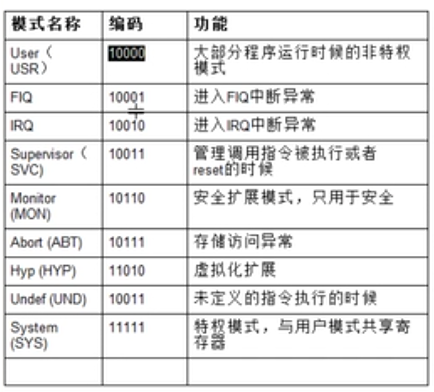
\includegraphics[scale=0.8]{arm_models.png}
  \caption{ARM的运行模式}
  \label{fig:arm_arch}
\end{figure}

ARM还拥有18个寄存器,每个寄存器长度为32位,R0~R12为通用寄存器,R13为栈指针寄存器(SP),R14为
链接指针寄存器(LP),R15为程序计数器(PC),如下图\nameref{fig:arm_reg}所示
\begin{figure}[H]
  \centering
  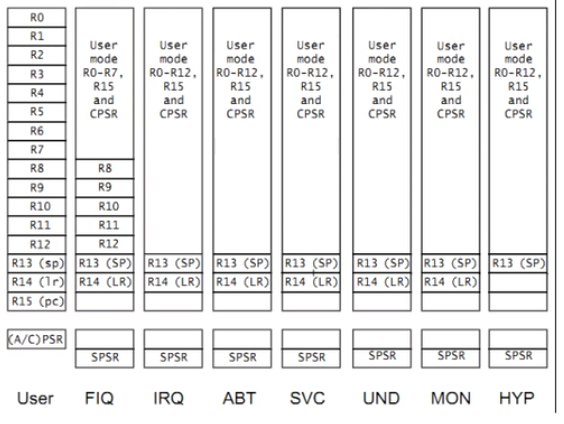
\includegraphics[scale=0.6]{arm_reg.png}
  \caption{ARM寄存器分类}
  \label{fig:arm_reg}
\end{figure}

除了这16个寄存器之外,ARM根据模式的不同,还有APSR(应用程序寄存器)/CPSR(当前程序寄存器)和SPSR(已存储程序寄存器)。
R0-R12寄存器,在所有模式(除快速中断模式)当中共享;快速中断(通常与硬件相关,FIQ)独占R8~R12寄存器;PC和CPSR寄存器是所有模式共享;
其余的寄存器基本是每种模式自己独占;用户模式(Usr)下不存在SPSR。

每一条ARM指令都是32位长度的,CPSR指令的格式大致如下图\nameref{fig:arm_command}所示:
\begin{figure}[H]
  \centering
  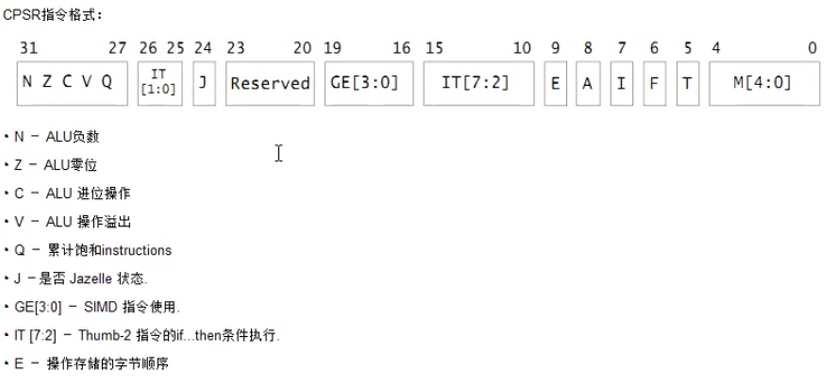
\includegraphics[width=\linewidth]{arm_command.png}
  \caption{ARM指令}
  \label{fig:arm_command}
\end{figure}

其中,指令的最后5位(M[4:0])正好表示本条指令的运行模式;第5位T,表示该指令是否使用是
Thumb指令集,1表示使用;第6位F表示FIQ,表示是否禁用FIQ中断;第7位I表示是否禁用IRQ;
第8位A表示是否禁用异步的abort;第9位E表示操作的字节序,即大小端;10-15位(IT[7:2])表示
Thumb2指令集当中的if-then条件执行;16-19位(GE[3:0])表示SIMD指令(单指令多数据);20-23位
为保留位;24位J表示Jazell状态,是否启用java加速;25-26(IT[1:0])表示Thumb指令集当中的if-then;
27到31分别为Q(累计饱和),V(ALU操作溢出),C(ALU进位操作),Z(ALU零位),N(ALU负数)。

\section{OpenCV交叉编译}
OpenCV是广泛使用的图形图像处理的C/C++函数库,在嵌入式当中,也使用非常广泛。但是,
嵌入式的计算性能毕竟有限,因此,在嵌入式设备上进行OpenCV的编译是非常耗时的。通常采用
交叉编译的方式进行OpenCV的编译,然后再将其移植到ARM等嵌入式设备上,具体操作如下:
\footnote{来源:\url{http://www.studiow.cf/blog/post/how-to-cross-compile-opencv-for-armbian-with-gtk}

\url{https://gist.github.com/Garrus007/6e43211c7a48b4f8600efc6d86d44703}}。

\begin{outline}[enumerate]

\1 安装交叉编译工具链

交叉编译的环境通常在X86的虚拟机或者服务器上,这样能够保证编译的时间。必须注意的是,
由于OpenCV编译完成之后,大多数是so文件,而so文件属于运行时的文件,因此,交叉编译环境
的ldd必须与嵌入式平台的版本一致,否则即使编译完成,也无法进行运行。比较好的做法是,
保持交叉编译环境的操作系统版本和开发板所运行的操作系统版本一致。
\begin{code-in-enumerate}{bash}
apt-get install gcc-arm-linux-gnueabihf g++-arm-linux-gnueabihf \
    pkg-config-arm-linux-gnueabihf -y
\end{code-in-enumerate}

\1 连接嵌入式平台

交叉编译环境上,有很多的类库以及依赖文件,是X86平台上没有或者不匹配的,因此,
我们通过远程连接的方式,将远程的嵌入式平台的操作系统链接到交叉编译环境中。假设
嵌入式平台的ip为172.16.1.155,则操作如下:
\begin{code-in-enumerate}{bash}
sshfs root@172.16.1.155:/ /mnt -o transform_symlinks -o allow_other
\end{code-in-enumerate}

\1 链接嵌入式平台上的开发库以及相关文件

在X86平台上,直接将嵌入式平台上的开发库文件链接到X86本地,方便进行编译开发。
\begin{code-in-enumerate}{bash}
ln -s /mnt/usr/lib/arm-linux-gnueabihf/ /usr/lib/arm-linux-gnueabihf
ln -s /mnt/lib/arm-linux-gnueabihf/ /lib/arm-linux-gnueabihf
ln -s /mnt/usr/share /usr/share/arm-linux-gnueabihf
ln -s /mnt/usr/include/arm-linux-gnueabihf /usr/include/arm-linux-gnueabihf
\end{code-in-enumerate}

注意,由于是通过远程挂载的方式进行交叉编译,因此,需要在嵌入式平台(ARM)上进行
编译所需要的依赖关系的安装。
\begin{code-in-enumerate}{bash}
apt-get install libjpeg-dev libtiff5-dev libjasper-dev libpng12-dev \
    libavcodec-dev libavformat-dev libswscale-dev libv4l-dev \
    libxvidcore-dev libx264-dev libgtk2.0-dev libatlas-base-dev \
    libglib2.0-dev gfortran python2.7-dev python3-dev ffmpeg libgtk-3-dev -y
\end{code-in-enumerate}

回到X86交叉编译环境,执行下面命令,以上面安装的libgtk2.0-dev为例:
\begin{code-in-enumerate}{bash}
arm-linux-gnueabihf-pkg-config --list-all | grep gtk
arm-linux-gnueabihf-pkg-config --libs gtk+-2.0
arm-linux-gnueabihf-pkg-config --cflags gtk+-2.0
\end{code-in-enumerate}
如果出现下面图\nameref{fig:cross_cv}的显示,则说明交叉编译的依赖关系没有问题了,可以进行编译了。
\begin{figure}[H]
  \centering
  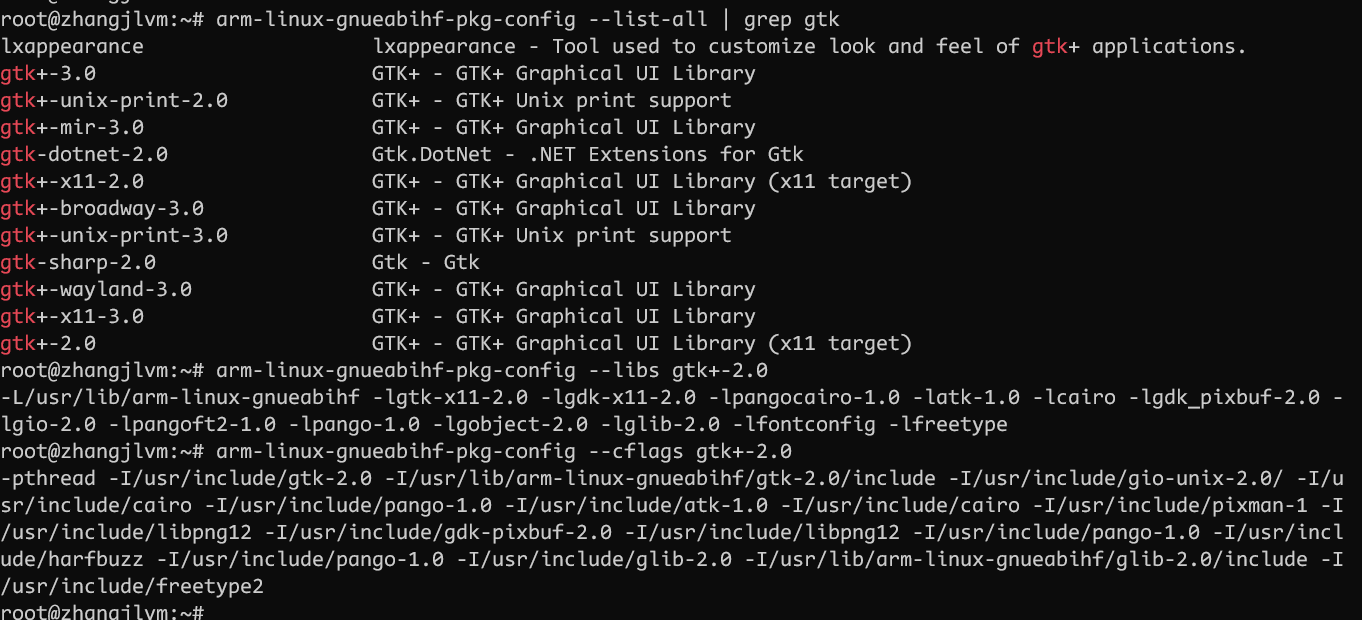
\includegraphics[width=\linewidth]{cross_cv.png}
  \caption{交叉编译的类库}
  \label{fig:cross_cv}
\end{figure}

如果提示错误,则需要按照下面的操作进行:
\begin{code-in-enumerate}{bash}
export PKG_CONFIG_SYSROOT_DIR=/mnt
export PKG_CONFIG_PATH=/usr/share/arm-linux-gnueabihf/pkgconfig:/mnt/usr/lib/pkgconfig
arm-linux-gnueabihf-pkg-config --libs gtk+-2.0
arm-linux-gnueabihf-pkg-config --cflags gtk+-2.0
\end{code-in-enumerate}

\1 下载代码

需要下载OpenCV和OpenCV-Contrib的代码,进行完整编译和模块编译。
\begin{code-in-enumerate}{bash}
git clone https://github.com/opencv/opencv.git
cd opencv && git checkout 3.2.0 && cd
git clone https://github.com/opencv/opencv_contrib.git
cd opencv_contrib && git checkout 3.2.0 && cd ../opencv
\end{code-in-enumerate}

\1 编译代码

首先需要准备编译目录,假设命名为build\_arm
\begin{code-in-enumerate}{bash}
cd opencv
mkdir build_arm
cd build_arm
\end{code-in-enumerate}

修改编译链工具文件
\begin{code-in-enumerate}{bash}
vi ../platforms/linux/arm-gnueabi.toolchain.cmake
\end{code-in-enumerate}

在该文件开始的地方,加入以下的代码:
\begin{code-in-enumerate}{bash}
set(ENV{PKG_CONFIG_PATH} "/usr/share/arm-linux-gnueabihf/pkgconfig:/mnt/usr/lib/pkgconfig")
set(ENV{PKG_CONFIG_SYSROOT_DIR} "/mnt")
set(PKG_CONFIG_EXECUTABLE "/usr/bin/arm-linux-gnueabihf-pkg-config")
set(ENV{LD_LIBRARY_PATH} "/mnt/usr/lib")
set(ENV{C_INCLUDE_PATH} "/mnt/usr/include")
set(ENV{CPLUS_INCLUDE_PATH} "/mnt/usr/include")
\end{code-in-enumerate}

OpenCV3.2.0版本的分支还存在一个小小的bug,需要手动修复一下,否则会影响交叉编译。
修改opencv\_contrib/modules/freetype/CMakeLists.txt,将第22行修改为如下内容:
\footnote{来源:\url{https://github.com/opencv/opencv_contrib/pull/926}}。
\begin{code-in-enumerate}{bash}
ocv_define_module(freetype opencv_core opencv_imgproc PRIVATE_REQUIRED ${FREETYPE_LIBRARIES} ${HARFBUZZ_LIBRARIES} WRAP python)
\end{code-in-enumerate}

然后生成makefile文件:
\begin{code-in-enumerate}{bash}
cmake -DENABLE_NEON=ON -DENABLE_VFPV3=ON  -D WITH_V4L=ON  -D WITH_GTK=ON \
    -D CMAKE_BUILD_TYPE=Release -D BUILD_TESTS=OFF \
    -D CMAKE_TOOLCHAIN_FILE=/root/opencv/platforms/linux/arm-gnueabi.toolchain.cmake \
    /root/opencv/ -D OPENCV_EXTRA_MODULES_PATH=/root/opencv_contrib/modules ..
\end{code-in-enumerate}

OpenCV会默认安装在/usr/local下,如果需要更改安装路径,则需要在生成makefile的参数当中新增:
\begin{code-in-enumerate}{bash}
-D CMAKE_INSTALL_PREFIX=/opt/opencv #指定的路径
\end{code-in-enumerate}

如果cmake的信息当中,提示GUI没有支持,如图\nameref{fig:cross_gui}所示,一定要在嵌入式平台端安装GTK或者QT等图形化开发
的lib库,否则,OpenCV在运行时,将无法显示图像。
\begin{figure}[H]
  \centering
  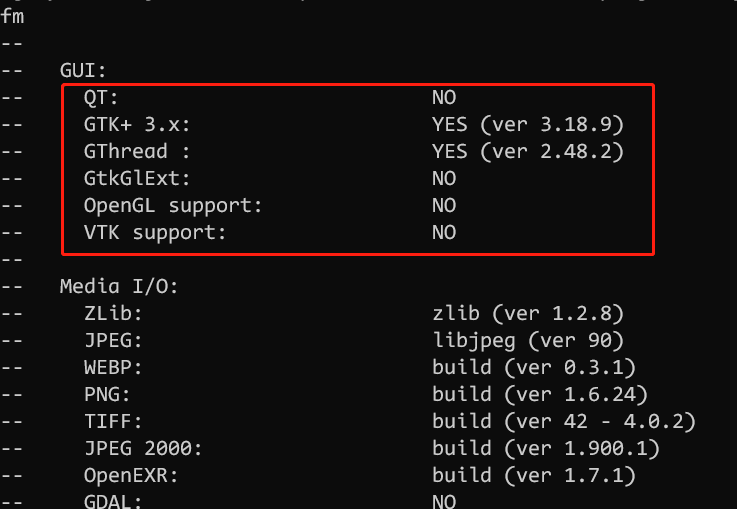
\includegraphics[scale=0.3]{cross_gui.png}
  \caption{图形化支持}
  \label{fig:cross_gui}
\end{figure}

随后进行OpenCV的编译:
\begin{code-in-enumerate}{bash}
make
make install
\end{code-in-enumerate}
如果一切顺利,将在opencv/build\_arm/install生成我们所需要的OpenCV文件,包括头文件,
so文件和其他的文件,大致如下图\nameref{fig:cross_finish}所示:
\begin{figure}[H]
  \centering
  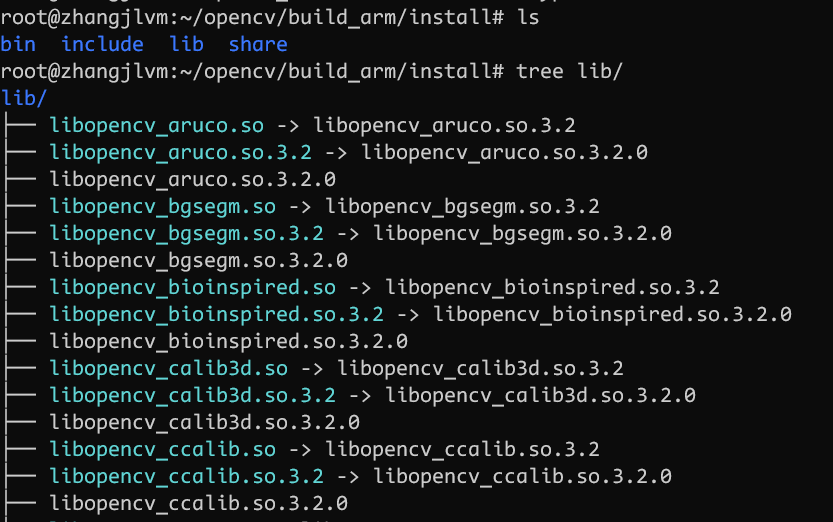
\includegraphics[width=\linewidth]{cross_finish.png}
  \caption{交叉编译的结果}
  \label{fig:cross_finish}
\end{figure}

然后将install下的所有文件,放到嵌入式系统的/usr/local当中对应的目录即可,注意,需要
修改install/lib/pkgconfig/opencv.pc文件,将prefix修改,修改为如下:
\begin{code-in-enumerate}{bash}
prefix=/usr/local
\end{code-in-enumerate}

断开交叉编译环境与嵌入式系统的文件链接:
\begin{code-in-enumerate}{bash}
fusermount -u /mnt
\end{code-in-enumerate}

完成上述操作之后,在嵌入式系统当中,执行指令:
\begin{code-in-enumerate}{bash}
ldconfig -v
\end{code-in-enumerate}

如果输出结果类似下面图\nameref{fig:cross_transplant}所示,则说明编译OpenCV移植成功,则ARM的嵌入式系统当中,可以正常使用。
\begin{figure}[H]
  \centering
  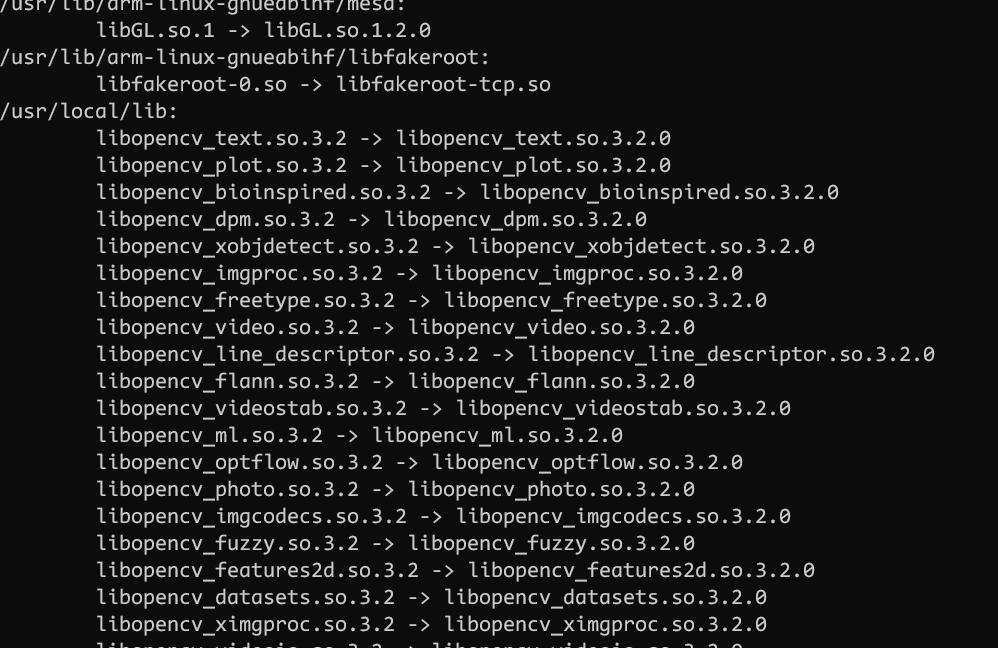
\includegraphics[width=\linewidth]{cross_transplant.png}
  \caption{移植到嵌入式系统}
  \label{fig:cross_transplant}
\end{figure}

\1 测试功能

移植之后,需要调用OpenCV的函数,才知道最终的结果。为此,我们编写一个简易的OpenCV应用程序,
只要能够将图片显示出来,就基本表明OpenCV的移植是没有问题的了。

代码的功能比较简单,就是读取一张图片,并显示出来,具体的代码如下:
\begin{code-in-enumerate}{cpp}
#include <opencv2/opencv.hpp>

using namespace cv;

int main(void)
{
        Mat img, gray;
        img = imread("lena.bmp", CV_LOAD_IMAGE_COLOR);
        imwrite("show", img);
        waitKey(0);
        destroyAllWindows();
        return 0;
}
\end{code-in-enumerate}

使用编译指令进行编译:
\begin{code-in-enumerate}{bash}
g++ -std=c++11 -Wall `pkg-config --cflags opencv` \
    -o canny canny.cc  `pkg-config --libs opencv` -lpthread
\end{code-in-enumerate}

也可以使用Makefile:
\begin{code-in-enumerate}{make}
TARGET = canny

CFLAGS = -Ofast -Wall -std=c++11 `pkg-config --cflags opencv`
LDFLAGS = -Ofast -Wall -std=c++11 `pkg-config --libs opencv`
CC = g++

all: $(TARGET)

$(TARGET): $(TARGET).o
        $(CC) $(LDFLAGS) -o $@ $^ `pkg-config --libs opencv` -lpthread

%.o: %.cpp
        $(CC) $(CFLAGS) -c -o $@ $<

clean:
        rm -f $(TARGET) *.a *.o *~
\end{code-in-enumerate}

执行该代码,如果该代码正常运行,且将图片正常显示,则表明OpenCV的移植没有任何
问题了,整个移植过程成功了。

\end{outline}

\section{构建ARM的rootfs}
首先是生成一个rootfs。
\begin{code-block}{bash}
apt-get install qemu-user-static
mkdir -p /opt/armhf-16.04-glibc-2.23
cd /opt/armhf-16.04-glibc-2.23
wget http://cdimage.ubuntu.com/ubuntu-base/releases/16.04/release/ubuntu-base-16.04.6-core-armhf.tar.gz
tar -zxvf ubuntu-base-16.04.6-core-armhf.tar.gz && rm -rf ubuntu-base-16.04.6-core-armhf.tar.gz
cp /usr/bin/qemu-arm-static usr/bin
cp /etc/resolv.conf etc/resolv.conf
\end{code-block}

创建一个脚本,用于进入rootfs环境,脚本内容大致如下:
\begin{code-block}{bash}
#!/bin/bash
function mnt() {
    echo "MOUNTING"
    sudo mount -t proc /proc ${2}proc
    sudo mount -t sysfs /sys ${2}sys
    sudo mount -o bind /dev ${2}dev
    sudo mount -o bind /dev/pts ${2}dev/pts
    sudo chroot ${2} /bin/bash --login
}

function umnt() {
    echo "UNMOUNTING"
    sudo umount ${2}proc
    sudo umount ${2}sys
    sudo umount ${2}dev/pts
    sudo umount ${2}dev
}

if [ "$1" == "-m" ] && [ -n "$2" ] ;
then
    mnt $1 $2
elif [ "$1" == "-u" ] && [ -n "$2" ];
then
    umnt $1 $2
else
    echo ""
    echo "Either 1'st, 2'nd or both parameters were missing"
    echo ""
    echo "1'st parameter can be one of these: -m(mount) OR -u(umount)"
    echo "2'nd parameter is the full path of rootfs directory(with trailing '/')"
    echo ""
    echo "For example: ch-mount -m /media/sdcard/"
    echo ""
    echo 1st parameter : ${1}
    echo 2nd parameter : ${2}
fi
\end{code-block}

执行该脚本,进入rootfs环境:
\begin{code-block}{bash}
./ch-mount -m /opt/armhf-16.04-glibc-2.23
\end{code-block}

升级rootfs,并安装必要的软件包:
\begin{code-block}{bash}
apt-get update -y && apt-get upgrade -y
apt-get install vim pkg-config git sudo ssh net-tools ethtool wireless-tools \
    lxde xfce4-power-manager xinit xorg network-manager iputils-ping rsyslog \
    lightdm-gtk-greeter alsa-utils lightdm bash-completion lxtask htop \
    python-gobject-2 python-gtk2 synaptic libjpeg-dev libtiff5-dev libjasper-dev \
    libpng12-dev libavcodec-dev libavformat-dev libswscale-dev libv4l-dev \
    libxvidcore-dev libx264-dev libgtk2.0-dev libatlas-base-dev libglib2.0-dev \
    gfortran libgtk-3-dev gcc cmake ifupdown qt5-default -y
\end{code-block}

添加必要的服务:
\begin{code-block}{bash}
echo "auto eth0" > /etc/network/interfaces.d/eth0
echo "iface eth0 inet dhcp" >> /etc/network/interfaces.d/eth0
echo "127.0.0.1    localhost.localdomain localhost" > /etc/hosts
echo "127.0.0.1    armhf" >> /etc/hosts
\end{code-block}

退出rootfs环境:
\begin{code-block}{bash}
exit
/opt/ch-mount -u /opt/armhf-16.04-glibc-2.23
rm -rf /opt/armhf-16.04-glibc-2.23/usr/bin/qemu-arm-static
\end{code-block}

当然也可以使用ubuntu的其他版本进行rootfs的编译和生成,其具体过程与上述类似,只是,
在ubuntu16.04之后,不再提供core版本的rootfs,因此,如果是使用ubuntu18.04或者其他更新的
版本,则需要在其中安装一些其他的软件,否则,制作的rootfs将无法引导开发板进行启动。
\begin{code-block}{bash}
apt-get install net-tools ethtool wireless-tools network-manager \
    ifupdow util-linux sysvinit-utils init-system-helpers \
    init systemd openssh-server
\end{code-block}

基本到此处,整个rootfs已经定制完成。当然,还可以根据需要,添加用户,修改用户密码等。

除了使用ubuntu作为rootfs,在嵌入式的领域,还可以使用busybox,yocto等,这些是轻量级的rootfs,
在嵌入式领域以及实时领域使用非常广泛。简单介绍一下busybox的编译过程。
\begin{code-block}{bash}
git clone https://github.com/buildroot/buildroot
cd buildroot
git checkout 2019.11.2
export CROSS_COMPILE=/opt/gcc-linaro-7.5.0-2019.12-x86_64_arm-linux-gnueabihf/bin/arm-linux-gnueabihf-
make -C . ARCH=ARM BR2_TOOLCHAIN_EXTERNAL_PATH=/opt/gcc-linaro-7.5.0-2019.12-x86_64_arm-linux-gnueabihf/
nconfig
\end{code-block}
进入Target options菜单,如下图\nameref{fig:buildroot}所示:
\begin{figure}[H]
  \centering
  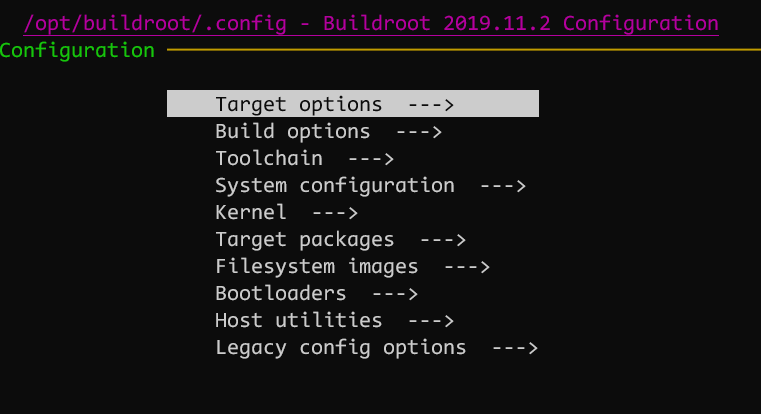
\includegraphics[width=\linewidth]{buildroot.png}
  \caption{编译菜单}
  \label{fig:buildroot}
\end{figure}
选择Target Architecture为ARM(little endian),
Target Architecture Variant为cortex-A9,启用Enable NEON SIMD extension support和
Enable VFP extension support,选择Target ABI为EABIhf,Floating point strategy为
NEON,如下图\nameref{fig:target_options}所示:
\begin{figure}[H]
  \centering
  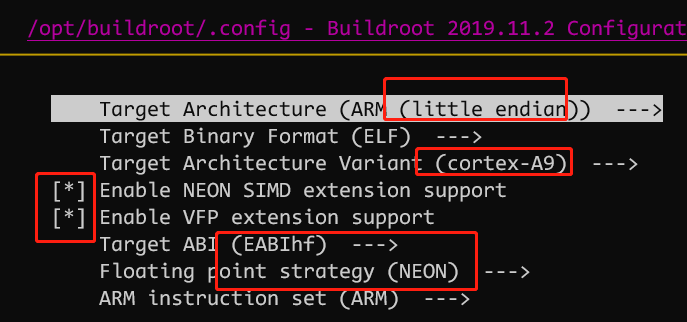
\includegraphics[width=\linewidth]{target_options.png}
  \caption{目标选项}
  \label{fig:target_options}
\end{figure}
选择Toolchain,进行工具链的选择,如下图\nameref{fig:toolchain}所示:
\begin{figure}[H]
  \centering
  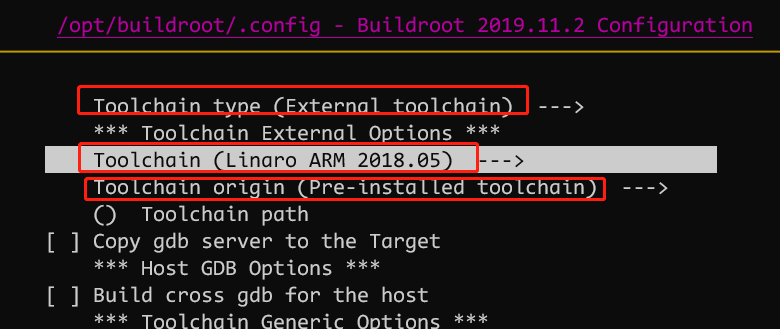
\includegraphics[width=\linewidth]{toolchain.png}
  \caption{工具链}
  \label{fig:toolchain}
\end{figure}

选择System configuration,进行主机名和密码的设置,如下图\nameref{fig:sys_config}所示:
\begin{figure}[H]
  \centering
  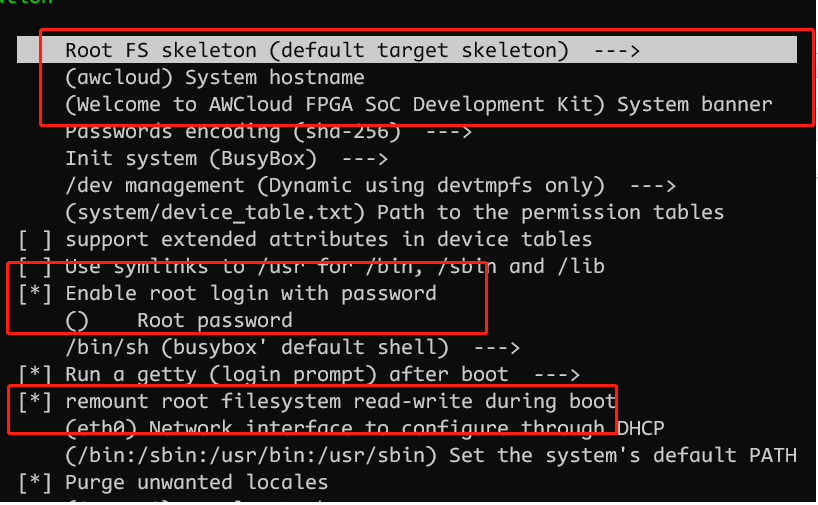
\includegraphics[width=\linewidth]{sys_config.png}
  \caption{系统配置}
  \label{fig:sys_config}
\end{figure}

其余选项可以忽略。然后按F6进行保存,保存完毕之后,F9推出,然后进行编译:
\begin{code-block}{bash}
make -C . BR2_TOOLCHAIN_EXTERNAL_PATH=/opt/gcc-linaro-7.5.0-2019.12-x86_64_arm-linux-gnueabihf/ all
\end{code-block}
编译成功之后,会在output/images生成我们所需要的rootfs.tar文件。

到此,不管是ubuntu的rootfs,还是busybox的rootfs,我们都算是编译完成了。这里额外的说一句,
Redhat/CentOS系列主要的重心在服务器领域,相对而言,在嵌入式领域较少,因此,暂时还无法进行
Redhat系列的rootfs的编译。编译完成的rootfs,需要封装到镜像文件当中,然后烧录到SD卡上,
才能够用于启动开发板。

rootfs的烧录使用的是一个脚本文件,脚本文件的内容如下:
\begin{code-block}{python}
#!/usr/bin/env python
#
# Copyright (c) 2014, Altera Corporation
# All rights reserved.
#
# Redistribution and use in source and binary forms, with or without
# modification, are permitted provided that the following conditions are met:
#
#     * Redistributions of source code must retain the above copyright
#       notice, this list of conditions and the following disclaimer.
#     * Redistributions in binary form must reproduce the above copyright
#       notice, this list of conditions and the following disclaimer in the
#       documentation and/or other materials provided with the distribution.
#     * Neither the name of Altera Corporation nor the
#       names of its contributors may be used to endorse or promote products
#       derived from this software without specific prior written permission.
#
# THIS SOFTWARE IS PROVIDED BY THE COPYRIGHT HOLDERS AND CONTRIBUTORS "AS IS" AND
# ANY EXPRESS OR IMPLIED WARRANTIES, INCLUDING, BUT NOT LIMITED TO, THE IMPLIED
# WARRANTIES OF MERCHANTABILITY AND FITNESS FOR A PARTICULAR PURPOSE ARE
# DISCLAIMED.  IN NO EVENT SHALL ALTERA CORPORATION BE LIABLE FOR ANY
# DIRECT, INDIRECT, INCIDENTAL, SPECIAL, EXEMPLARY, OR CONSEQUENTIAL DAMAGES
# (INCLUDING, BUT NOT LIMITED TO, PROCUREMENT OF SUBSTITUTE GOODS OR SERVICES;
# LOSS OF USE, DATA, OR PROFITS; OR BUSINESS INTERRUPTION) HOWEVER CAUSED AND
# ON ANY THEORY OF LIABILITY, WHETHER IN CONTRACT, STRICT LIABILITY, OR TORT
# (INCLUDING NEGLIGENCE OR OTHERWISE) ARISING IN ANY WAY OUT OF THE USE OF THIS
# SOFTWARE, EVEN IF ADVISED OF THE POSSIBILITY OF SUCH DAMAGE.

import os
import sys
import re
import glob
import argparse
import textwrap
import subprocess
import time

MAX_PARTITIONS = 4

# Globals
loopback_dev_used = []
mounted_fs = []

def check_output(*popenargs, **kwargs):
    r"""Run command with arguments and return its output as a byte string.

    Backported from Python 2.7 as it's implemented as pure python on stdlib.

    >>> check_output(['/usr/bin/python', '--version'])
    Python 2.6.2
    """
    process = subprocess.Popen(stdout=subprocess.PIPE, *popenargs, **kwargs)
    output, unused_err = process.communicate()
    retcode = process.poll()
    if retcode:
        cmd = kwargs.get("args")
        if cmd is None:
            cmd = popenargs[0]
            error = subprocess.CalledProcessError(retcode, cmd)
            error.output = output
        raise error
    return output

#==============================================================================
# Convert to bytes
def convert_size_from_unit(unit_size):

    factor = 1

    m = re.match("^[0-9]+[KMG]?$", unit_size, re.I)
    if m == None:
        print "error: "+unit_size+": malformed expression"
        sys.exit(-1)
    else:
        munit = re.search("[KMG]+$", m.group(0), re.I)
        msize = re.search("^[0-9]+", m.group(0), re.I)

        if munit :
            unit = munit.group(0).upper()

            if unit == 'K':
                factor = 1024
            elif unit == 'M':
                factor = 1024*1024
            elif unit == 'G':
                factor = 1024*1024*1024

    # convert_str_to_int() takes care of handling exceptions
    size = convert_str_to_int(msize.group(0))*factor

    return size

#==============================================================================
# converts a string to int, with exception handling
def convert_str_to_int(string):

    try:
        integer = int(string)

    except ValueError:
        print "error: "+string+": not a valid number"
        sys.exit(-1)

    return integer

#==============================================================================
# Checks the requested file system format is supported
def validate_format(fs_format):

    match = re.search("^(ext[2-4]|xfs|fat32|vfat|fat|none|raw)$", fs_format, re.I)
    if match:
        return True
    else:
        return False

#==============================================================================
# The switch '-P' can be used multiple times, this function checks one
# instance
# It returns a dictionary with the right entries
def parse_single_part_args(part):

    part_entries = {}
    part_entries['files'] = []

    p = re.compile("[a-zA-Z0-9]+=")

    for el in part.split(","):
        if p.match(el):
            key, value = el.split("=")
            #  need to test for a situation like key=, that is
            #! without a value.
            if value == None:
                print "error: "+key+": no value found."
                sys.exit(-1)

            # check that a valid key was used
            if key == 'num':
                part_entries[key] = convert_str_to_int(value)
            elif key == 'size':
                size = convert_size_from_unit(value)
                part_entries[key] = size
            elif key == 'format':
                if validate_format(value):
                    part_entries[key] = value
                else:
                    print "error:", value, "unknown format"
                    sys.exit(-1)
            elif key == 'type':
                part_entries[key] = value
            else:
                print "error:", key,": unknown option"
                sys.exit(-1)
        else:
            part_entries['files'].append(el)

    return part_entries

#==============================================================================
# Parse all the arguments provided with all the '-P' switches
def parse_all_parts_args(part_args):

    part_entries = {}

    num_args = len(part_args)
    if num_args > MAX_PARTITIONS:
        print "error: up to "+str(MAX_PARTITIONS)+" allowed"
        sys.exit(-1)

    for part in part_args:
        part_entry = parse_single_part_args(part)
        if part_entry['num'] in part_entries.keys():
            print "error:"+str(part_entry['num'])+": partition already used"
            sys.exit(-1)

        part_entries[part_entry['num']] = part_entry

    return part_entries

#==============================================================================
# in some cases, a partition type (fdisk) can be inferred from the file system
# format, e.g. ext[2-4], type=83
def derive_fdisk_type_from_format(pformat):

    ptype = ""

    if re.match('^ext[2-4]|xfs$', pformat):
        ptype = '83'
    elif re.match('^vfat|fat|fat32$', pformat):
        ptype = 'b'
    else:
        print "error:", pformat,": unknown format"
        sys.exit(-1)

    return ptype

#==============================================================================
# The partition type provided by the user is not in the format that fdisk
# expects. This function translates to fdisk type defs
def derive_fdisk_type_from_ptype(ptype):

    ptype = ""

    if re.match('^raw|none$', ptype):
        fdisk_type = 'A2'
    elif ptype == 'swap':
        fdisk_type = '84'
    else:
        print "error:", ptype,": unknown type"
        sys.exit(-1)

    return fdisk_type

#==============================================================================
# This function checks the partition definitions and calculates the
# partition offsets
def check_and_update_part_entries(part_entries, image_size):

    entry = {}
    offset = 2048   # in blocks of 512 bytes
    total_size = 0


    for part in part_entries.keys():

        entry = part_entries[part]

        # we need to check if num, size and format are set
        # if type is not set but format is set, we can derive the type
        # as long as the format is not 'raw' or 'none'
        if 'size' not in entry:
            print "error:", part, ": size must be specified"
            sys.exit(-1)
        if entry['size'] == 0:
            print "error:", part, ": size is 0"
            sys.exit(-1)
        total_size = total_size + entry['size']

        if 'format' not in entry:
            if 'type' not in entry:
                print "error:", part,": specify at least format or type"
                sys.exit(-1)

            part_entries[part]['fdisk_type'] = derive_fdisk_type_from_ptype(
                entry['type'])

        else: # format in  entry
            if 'type' not in entry:
                part_entries[part]['fdisk_type'] = derive_fdisk_type_from_format(
                    entry['format'])
            else:
                part_entries[part]['fdisk_type'] = entry['type']

        # update offset
        part_entries[part]['start'] = offset # in sectors
        # because size is in bytes
        bsize = ( entry['size'] / 512 + ((entry['size'] % 512) != 0)*1)
        offset = offset + bsize + 1

        # it is handy to save the size in blocks, as this is what fdisk needs
        part_entries[part]['bsize'] = bsize

    if total_size > image_size:
        print "error: partitions are too big to fit in image"
        sys.exit(-1)

    return part_entries

#==============================================================================
# this script can only be run by the zuper user
def is_user_root():

    return (os.getuid() == 0)

#==============================================================================
# check if a file exists
def check_file_exists(filename):

    return os.path.isfile(filename)

#==============================================================================
# this function creates an empty image
def create_empty_image(image_name, image_size, force_erase_image):

    # first check if the image exists...
    if check_file_exists(image_name):
        if force_erase_image == False:
            yes_or_no = raw_input(
                "the image "+image_name+" exists. Remove? [y|n] ")
        else:
            yes_or_no = 'Y'

        if yes_or_no == 'Y' or yes_or_no == 'y':
            try:
                os.remove(image_name)
            except OSError:
                print "error: failed to remove "+image_name+". Exit"
                sys.exit(-1)
            print "image removed"

        else:
            print "user declined"
            return False

    # now we can proceed with the image creation
    # we'll create an empty image to speed things up...
    try:
        check_output(["dd", "if=/dev/zero", "of="+image_name,"bs=1",
                                 "count=0", "seek="+str(image_size)],
                                stderr=subprocess.STDOUT)
    except subprocess.CalledProcessError:
        print "error: failed to create the image"
        sys.exit(-1)

    return True

#==============================================================================
# this function creates a loopback device
# it is assumed the file exists
# offset in bytes
def create_loopback(image_name, size, offset=0):

    try:
        if offset != 0:
            device = check_output(
                  ["losetup", "--show", "-f", "-o "+str(offset),
                   "--sizelimit", str(size), image_name])
        else:
            device = check_output(
                        ["losetup", "--show", "-f",
                         "--sizelimit", str(size), image_name])
    except subprocess.CalledProcessError:
        print "error: failed to get a loopback device"
        clean_up()
        sys.exit(-1)

    # strip trailing \n
    device = str.rstrip(device)
    # keep track of the devices used
    loopback_dev_used.append(device)

    return device

#==============================================================================
# this function deletes a loopback device
def delete_loopback(device):

    try:
        check_output(["losetup", "-d", str(device)], stderr=subprocess.STDOUT)
    except subprocess.CalledProcessError:
        return False

    # remove the device from the list
    loopback_dev_used.remove(device)

    return True

#==============================================================================
# clean up
def clean_up():

    for mp in mounted_fs:
        umount_fs(mp)

    for device in loopback_dev_used:
        if not delete_loopback(device):
            print "error: could not delete loopback device", device


    return 0

#==============================================================================
# this function creates the partition table
def create_partition_table(loopback, partition_entries):

    # our command list for fdisk
    cmd = ""
    # the number of questions asked bby fdisk, for one partition depebds
    #!on the number of partitions defined
    first_part = True

    cmds = []
    for part in partition_entries.keys():
        pentry = partition_entries[part]
        cmds.append('n\np\n')
        cmds.append(str(pentry['num']) +'\n')
        cmds.append(str(pentry['start']) +'\n')
        cmds.append('+'+str(pentry['bsize']) + '\n')
        if first_part:
            cmds.append('\nt\n')
            cmds.append(pentry['fdisk_type']+'\n')
            first_part = False
        else:
            cmds.append('\nt\n')
            cmds.append(str(pentry['num']) + '\n')
            cmds.append(pentry['fdisk_type'] + '\n')

    cmds.append('\nwq\n')

    printargs = ''.join(cmds)
    p1=subprocess.Popen(['printf',printargs],
        stdout=subprocess.PIPE, stderr=subprocess.PIPE)
    p=subprocess.Popen(['fdisk',loopback], stdin=p1.stdout,
        stderr=subprocess.PIPE, stdout= subprocess.PIPE).wait()

    # we need to write and quit

    ## sometimes the kernel does not reload the pattition table
    ##!a little help is needed
    #if p!= 0:
    #    pp = subprocess.Popen(["partprobe", loopback])
    #    pp.wait()
    #    if pp.returncode != 0:
    #        print "error: could not reload the partition table from image"
    #        sys.exit(-1)
    return

#==============================================================================
# map format to a command
def get_mkfs_from_format(pformat):

    cmd = ""

    if re.search("^ext[2-4]$", pformat):
        cmd = "mkfs."+pformat
    elif re.search("fat|vfat|fat32", pformat):
        cmd = "mkfs.vfat"
    elif re.search("^xfs$", pformat):
        cmd = "mkfs.xfs"

    return cmd

#==============================================================================
# map format to a command parameter
def get_mkfs_params_from_format(pformat):

    params = ""

    if re.search("fat32", pformat):
        params = "-F 32"

    return params

#==============================================================================
# formats a vlock device
def format_partition(loopback, fs_format):

    cmd = get_mkfs_from_format(fs_format)
    params = get_mkfs_params_from_format(fs_format)
    if cmd:
        if params:
            p = subprocess.Popen([cmd, loopback, params],
                                 stdout=subprocess.PIPE, stderr=subprocess.PIPE)
        else:
            p = subprocess.Popen([cmd, loopback],
                                 stdout=subprocess.PIPE, stderr=subprocess.PIPE)
        #RODO: add timeout?
        p.wait()
        if p.returncode != 0:
            print "error: format: failed"
            #clean_up()
            #sys.exit(-1)

    return

def get_mountfs_from_format(pformat):
    format = pformat

    if re.search("fat32|fat", pformat):
        format = "vfat"

    return format
#==============================================================================
# mount a file system
#! returns the mnt point
def mount_fs(loopback, fs_format):

    mp = "/tmp/"+str(int(time.time()))+"_"+str(os.getpid())
    try:
        os.mkdir(mp)
    except OSError:
        print "error: failed to create mount point (", mp,")"
        clean_up()
        sys.exit(-1)

    format = get_mountfs_from_format(fs_format)

    p = subprocess.Popen(["mount", "-t", format, loopback, mp],
                         stdout=subprocess.PIPE, stderr=subprocess.PIPE)
    p.wait()
    if p.returncode != 0:
        print "error: mount: failed (", loopback, mp,")"
        clean_up()
        sys.exit(-1)

    # keep track of the mount points
    mounted_fs.append(mp)

    return mp

#==============================================================================
# unmount fs
def umount_fs(mp):

    time.sleep(3)
    p = subprocess.Popen(["umount", mp],
                         stdout=subprocess.PIPE, stderr=subprocess.PIPE)
    p.wait()
    if p.returncode != 0:
        print "error: failed to umount", mp
        sys.exit(-1)

    # update the list
    mounted_fs.remove(mp)

    return

#==============================================================================
#do a raw copy of files to a partition
def do_raw_copy(loopback, partition_data):

    offset = 0  # offset in bytes

    # below, stuff is just a file...
    for stuff in partition_data['files']:
        # we do accept FILES only, no directories please
        if os.path.isdir(stuff):
            print "error:", stuff, ": can't copy dirs to raw partitions"
            clean_up()
            sys.exit(-1)

        # now dd the file:
        #! dd if=file of=loopback bs=1 seek=offset
        p = subprocess.Popen(["dd", "if="+stuff, "of="+loopback, "bs=1",
                             "seek="+str(offset)],
                             stdout=subprocess.PIPE, stderr=subprocess.PIPE)
        p.wait()
        if p.returncode != 0:
            print "error:", stuff, ": failed to do raw copy"
            clean_up()
            sys.exit(-1)

        # handle offset
        offset = offset + os.stat(stuff).st_size

    return

#==============================================================================
# copy files over a file system
def do_copy(loopback, partition_data):

    mp = mount_fs(loopback, partition_data['format'])
    for stuff in partition_data['files']:
        if os.path.isdir(stuff):
            stuff = stuff+"/*"

        # some file systems have limited flags like FAT
        if re.search("^fat|vfat|fat32$", partition_data['format']):
            cp_opt = "-rt"
        else:
            cp_opt = "-at"

        # as we need to do UNIX path expansion, we'll use the class glob,
        #! so we need to call cp with the option -t, such that the destination
        #! directory can be specified first. The list returned by glob can then
        #! be added to the list of args passed to Popen
        try:
            p = subprocess.Popen(["cp", cp_opt, mp ] + glob.glob(stuff),
                                 stdout=subprocess.PIPE, stderr=subprocess.PIPE)
            p.wait()
            if p.returncode:
                raise Exception([])
        except Exception:
            print "error: failed to copy", stuff
            clean_up()
            sys.exit(-1)

    umount_fs(mp)

    return

#==============================================================================
# copy files to  a partition
#! takes care of the format, if raw|none use dd
def copy_files_to_partition(loopback, partition_data):

    if re.search("raw|none", partition_data['format']):
        # RAW patition, nothin to mount, the files must be
        #! dd'ed in. ONLY files allowed, no directory
        # if multiple files are provided, they are dd'ed one after another,
        #! no GAP. If not acceptable, one file should be passed, as an image
        do_raw_copy(loopback, partition_data)
    else:
        do_copy(loopback, partition_data)

    return

#==============================================================================
# create, formats and copt files to partition
def do_partition(partition, image_name):

    offset_bytes = partition['start'] * 512

    if partition['format'] == "fat32" and partition['size'] < 33554432:
        print "error: Unable to create a fat32 partition size < 32MB"
        sys.exit(-1)

    loopback = create_loopback(image_name, partition['size'], offset_bytes)
    format_partition(loopback, partition['format'])
    copy_files_to_partition(loopback, partition)
    time.sleep(3)
    if not delete_loopback(loopback):
        clean_up()
        sys.exit(-1)

    return

#==============================================================================
def create_image(image_name, image_size, partition_entries, force_erase_image):

    print "info: creating the image "+image_name
    # first we need an empty image
    if not create_empty_image(image_name, image_size, force_erase_image):
        print "error: the image file could not be created"
        sys.exit(-1)

    # second, we'll create the partition table
    print "info: creating the partition table"
    loopback = create_loopback(image_name, image_size)
    create_partition_table(loopback, partition_entries)
    delete_loopback(loopback)

    # now we iterate over the partitions
    print "info: processing partitions..."
    for part in partition_entries.keys():
        print "     partition #"+str(part)+"..."
        do_partition(partition_entries[part], image_name)

    return

#==============================================================================
#==============================================================================
#
#   ####    #####    ##    #####    #####
#  #          #     #  #   #    #     #
#   ####      #    #    #  #    #     #
#       #     #    ######  #####      #
#  #    #     #    #    #  #   #      #
#   ####      #    #    #  #    #     #
#
part_entries = []

# arguments
parser = argparse.ArgumentParser(description='Creates an SD card image for Altera\'s SoCFPGA SoC\'s',
                                 epilog = textwrap.dedent('''\
Usage: PROG [-h] -P <partition info> [-P ...]
-P
'''
))
parser.add_argument('-P', dest='part_args', action='append',
                    help='''specifies a partition. May be used multiple times.
                            file[,file,...],num=<part_num>,format=<vfat|fat32|ext[2-4]|xfs|raw>,
                            size=<num[K|M|G]>[,type=ID]''')
parser.add_argument('-s', dest='size', action='store',
                    default='8G', help='specifies the size of the image. Units K|M|G can be used.')
parser.add_argument('-n', dest='image_name', action='store',
                    default='somename.img', help='specifies the name of the image.')
parser.add_argument('-f', dest='force_erase_image', action='store_true',
                    default=False, help='deletes the image file if exists')
args = parser.parse_args()

# Only root can do this
if not is_user_root():
    print "error: only root can do this..."
    sys.exit(-1)

# A few checks
part_entries = parse_all_parts_args(args.part_args)
image_size = convert_size_from_unit(args.size)
part_entries = check_and_update_part_entries(part_entries, image_size)

# we now have what we need
create_image(args.image_name, image_size, part_entries, args.force_erase_image)
print "info: image created, file name is ", args.image_name
\end{code-block}

执行的指令如下:
\begin{code-block}{python}
python make_sdimage.py -f \
    -P preloader-mkpimage.bin,u-boot.img,num=3,format=raw,size=10M,type=A2 \
    -P /opt /mksd/u16/*,num=2,format=ext4,size=1500M \
    -P zImage,u-boot.scr,soc_system.rbf,soc_system.dtb,num=1,format=fat32,size=500M \
    -s 2G -n u16.img
\end{code-block}

而生成的img文件,则可用于进行开发板的启动和引导。

\section{利用rootfs编译ARM的软件}
既然可以构建一个ARM的rootfs,这个rootfs当中,所有的类库都是armhf架构的,那是否可以
直接在rootfs当中编译ARM或者运行的软件?答案是肯定的。以编译ARM的OpenCV为例。

首先是进入ARM的rootfs,然后安装OpenCV相关的编译依赖包。退出rootfs,在X86的主机上,
下载OpenCV和OpenCV-Contribe的代码,统一放到/opt/opencv下,然后挂载到rootfs环境:
\begin{code-block}{bash}
bindfs -u root -g root -p +rw /opt/opencv/ /opt/arm-16.04-glibc-2.23/mnt
\end{code-block}

然后再次进入rootfs,按照前面所述,修改Opencv-Contrib的代码。注意,由于我们是在rootfs
下进行编译,该环境中的软件架构已经是ARM的了,因此,无需修改OpenCV的Cmake文件。紧接着开始进行
编译安装:
\begin{code-block}{bash}
cmake -DENABLE_NEON=ON -DENABLE_VFPV3=ON  -D WITH_V4L=ON  \
    -D WITH_GTK=ON -D CMAKE_BUILD_TYPE=Release -D BUILD_TESTS=OFF  \
    /mnt/opencv -D OPENCV_EXTRA_MODULES_PATH=/mnt/opencv_contrib/modules ..
make
make install
\end{code-block}

如果一切正常,在rootfs的/usr/local下,将生成相关的OpenCV文件。余下的操作和交叉编译OpenCV
的操作类似。

最后退出rootfs,并卸载相关的目录:
\begin{code-block}{bash}
umount /opt/arm-16.04-glibc-2.23/mnt
\end{code-block}

注意,该种编译方式的效率其实是比较低的,因此,大多数情况下,除非条件不允许,一般不推荐
使用rootfs的方式进行交叉编译。但是,也可以换一个思路:使用rootfs的文件,替换远程链接的嵌入式系统。
经过测试,使用rootfs替换远程链接的的方式进行编译(不使用chroot),功能上能够完全满足,编译时间
也能够完全控制在合理的范围内。

\section{编译自己的BSP}
SoC的BSP(即操作系统)通常需要根据自己的需要添加不同的功能或者模块,因此需要进行定制。以支持OpenCL,图形化以及USB相机
为例,进行BSP的编译。
\footnote{来源:\url{https://github.com/thinkoco/c5soc_opencl/tree/master/documents}}

\subsection{下载必要的代码}
\begin{code-block}{bash}
git clone https://github.com/thinkoco/c5soc_opencl.git
git clone https://github.com/thinkoco/c5soc_opencl_rte.git
git clone https://github.com/thinkoco/linux-socfpga.git thinkoco-linux-socfpga
cd thinkoco-linux-socfpga && git checkout origin/socfpga-4.9.78-aocl
\end{code-block}

由于内核代码有部分bug,需要进行部分的修改,修改如下:
\begin{code-block}{bash}
vi include/linux/fpga/fpga-mgr.h +110
# 修改为如下的模样:
u64 (*status)(struct fpga_manager *mgr);
\end{code-block}

\subsection{安装工具集}
需要安装的工具包括Quaruts18.1,\url{gcc-linaro-7.5.0-2019.12-x86\_64\_arm-linux-gnueabihf}。
假设Quartus安装在/opt/intelFPGA/18.1,gcc-linaro安装在\url{/opt/gcc-linaro-7.5.0-2019.12-x86\_64\_arm-linux-gnueabihf},
\begin{code-block}{bash}
cd c5soc_opencl
cp -rf de1soc_sharedonly_vga /opt/intelFPGA/18.1/hld/board/c5soc/hardware
cp -rf de10_nano_sharedonly_hdmi /opt/intelFPGA/18.1/hld/board/c5soc/hardware
cp -rf de10_standard_sharedonly_vga /opt/intelFPGA/18.1/hld/board/c5soc/hardware
\end{code-block}

编写环境变量文件,并设定:
\begin{code-block}{bash}
export QUARTUS_HOME=/opt/intelFPGA/18.1
export QSYS_ROOTDIR=/opt/intelFPGA/18.1/quartus/sopc_builder/bin
export INTELFPGAOCLSDKROOT=/opt/intelFPGA/18.1/hld
export QUARTUS_ROOTDIR=$QUARTUS_HOME/quartus
export QUARTUS_64BIT=1
export AOCL_BOARD_PACKAGE_ROOT=$INTELFPGAOCLSDKROOT/board/c5soc
export LD_LIBARY_PATH=$LD_LIBARY_PATH:$INTELFPGAOCLSDKROOT/host/arm32/lib
export PATH=$PATH:$QUARTUS_ROOTDIR/bin:$QUARTUS_HOME/embedded/ds-5/bin:$QUARTUS_HOME/embedded/ds-5/sw/gcc/bin:$INTELFPGAOCLSDKROOT/bin:$INTELFPGAOCLSDKROOT/host/arm32/bin
\end{code-block}

\subsection{生成rbf文件}
\begin{code-block}{bash}
mkdir sdcard
echo -e  "__kernel void hello_world(int thread_id_from_which_to_print_message) { \n\tunsigned thread_id = get_global_id(0);\n\tif(thread_id == thread_id_from_which_to_print_message) {\n\t\tprintf(\"Thread #%u: Hello from Altera's OpenCL Compiler! \\\n \", thread_id);\n\t}\n}" > hello_world.cl
aoc -report -v -o hello_world.aocx hello_world.cl -board=de10_standard_sharedonly_vga
cp hello_world/top.rbf sdcard/opencl.rbf
\end{code-block}

\subsection{生成u-boot文件}
\begin{code-block}{bash}
/opt/intelFPGA/18.1/embedded/embedded_command_shell.sh
cd hello_world
bsp-editor
\end{code-block}
选择“New HPS BSP”菜单,然后设置“Preloader settings directory”指向目标目录为hello\_world/hps\_isw\_handoff/system\_acl\_iface\_hps,
然后选择ok与生成,如下图\nameref{fig:bsp}所示:
\begin{figure}[H]
  \centering
  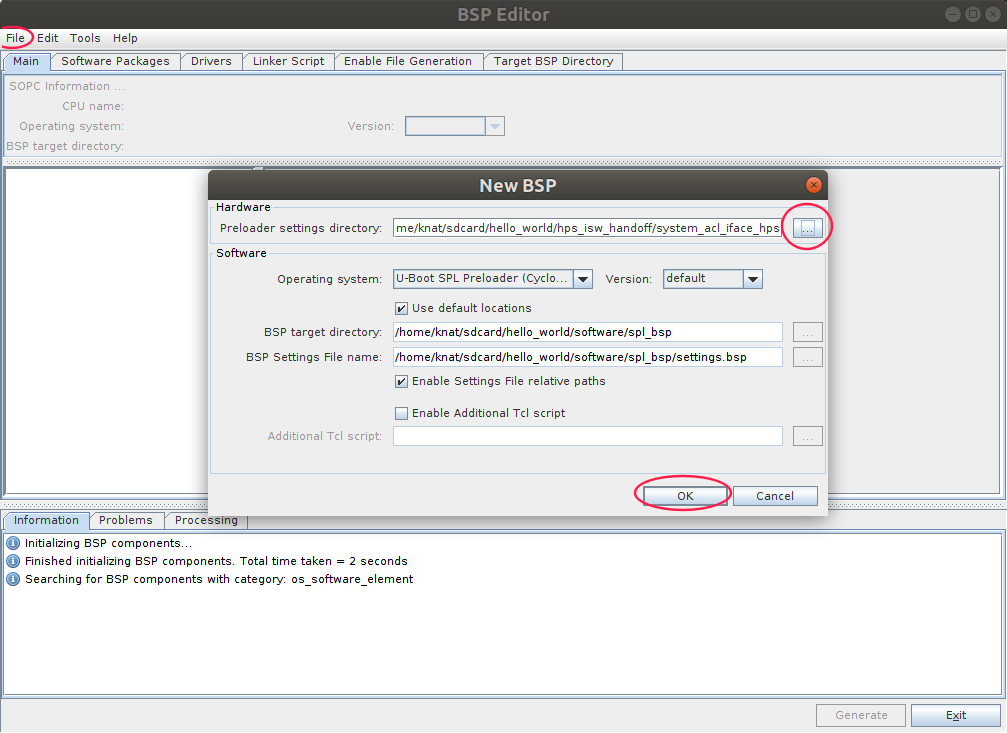
\includegraphics[width=\linewidth]{bsp.png}
  \caption{生成u-boot}
  \label{fig:bsp}
\end{figure}

然后进行后续操作:
\begin{code-block}{bash}
cd hello_world/software/spl_bsp/
make
cp preloader-mkpimage.bin ~/sdcard/
export CROSS_COMPILE=arm-linux-gnueabihf-
cd uboot-socfpga/
make
cp u-boot.img ~/sdcard/
\end{code-block}

生成u-boot配套文件:
\begin{code-block}{bash}
wget https://releases.rocketboards.org/release/2017.10/gsrd/src/boot.script
sed -i 's/soc_system/opencl/g' boot.script
mkimage   -A arm -O linux -T script -C none -a 0 -e 0 -n "My script" -d boot.script u-boot.scr
mv u-boot.scr ~/sdcard/
\end{code-block}

\subsection{编译内核}
\begin{code-block}{bash}
cd thinkoco-linux-socfpga
cp ../c5soc_opencl_rte/socfpga-4.9.78-ltsi/c5socl_defconfig .config
export ARCH=arm
export CROSS_COMPILE=/opt/gcc-linaro-7.5.0-2019.12-x86_64_arm-linux-gnueabihf/bin/arm-linux-gnueabihf-
export LOADADDR=0x8000
make menuconfig
\end{code-block}

勾选所有的USB摄像头驱动,如图\nameref{fig:usb_camera}所示:
\begin{figure}[H]
  \centering
  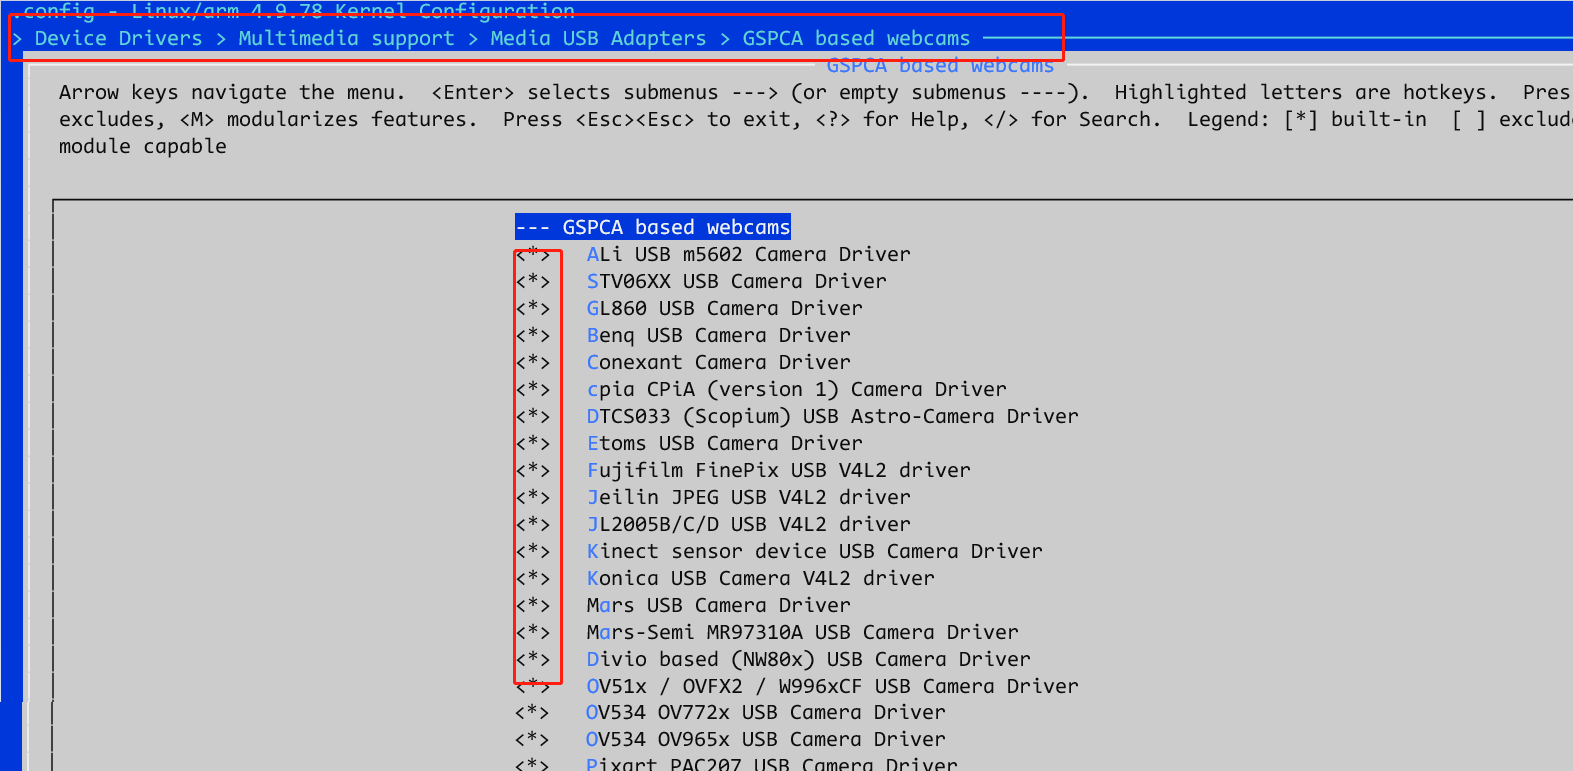
\includegraphics[width=\linewidth]{usb_camera.png}
  \caption{Usb摄像头驱动}
  \label{fig:usb_camera}
\end{figure}

然后进行编译:
\begin{code-block}{bash}
make zImage
make socfpga_cyclone5_de10_nano.dtb
make modules
make modules_install INSTALL_MOD_PATH=~/sdcard/
cp arch/arm/boot/zImage ~/sdcard
cp arch/arm/boot/dts/socfpga_cyclone5_de10_nano.dtb  ~/sdcard/socfpga.dtb
\end{code-block}

\subsection{编译rootfs}
\begin{code-block}{bash}
apt-get install qemu-user-static -y
mkdir sdcard/rootfs
wget http://cdimage.ubuntu.com/ubuntu-base/releases/18.04/release/ubuntu-base-18.04.4-base-armhf.tar.gz
tar -xvf  ubuntu-base-18.04.4-base-armhf.tar.gz -C rootfs/
cp /usr/bin/qemu-arm-static rootfs/usr/bin/
cp -r sdcard/lib/ rootfs
/ch-mount.sh -m rootfs/

echo nameserver 114.114.114.114 > /etc/resolv.conf
apt-get update
apt-get install language-pack-en-base vim sudo ssh net-tools ethtool wireless-tools \
    lxde xfce4-power-manager xinit xorg xserver-xorg-video-fbdev xserver-xorg-input-all \
    network-manager iputils-ping rsyslog lightdm-gtk-greeter alsa-utils mplayer lightdm \
    bash-completion lxtask htop python-gobject-2 python-gtk2 synaptic ifupdown
apt-get install locales-all tzdata resolvconf
echo "c5soc">/etc/hostname
echo "127.0.0.1 localhost" >> /etc/hosts
echo "127.0.1.1 c5soc" >> /etc/hosts

# Now add a user of your choice and include him in suitable groups
adduser knat && addgroup knat adm && addgroup knat sudo && addgroup knat audio
# set root without password
sed -i 's/^root\:\*/root\:/g' /etc/shadow
# modify getty@.service
sed -i 's/^ExecStart=-\/sbin\/agetty.*$/ExecStart=-\/sbin\/agetty --noclear %I $TERM/' /lib/systemd/system/getty@.service
# set lightdm.conf
echo -e "[SeatDefaults]\nautologin-user=root\nautologin-user-timeout=0" > /etc/lightdm/lightdm.conf
# set rc.local
echo -e '#!/bin/sh -e\n#\n# rc.local\n#\n#In order to enable or disable this script just change the execution bits\n\nmodprobe altvipfb\nservice lightdm start\n\nexit 0' > /etc/rc.local
chmod +x /etc/rc.local
# update DNS automatically,Set ‘timezone’,Make X used by ‘anyuser’
dpkg-reconfigure tzdata
dpkg-reconfigure resolvconf
dpkg-reconfigure x11-common
echo 'ACTION=="add|change", SUBSYSTEM=="block", ENV{UDISKS_IGNORE}="1"' > /etc/udev/rules.d/10-udisks.rules
exit
\end{code-block}

\subsection{编译opencl驱动}
\begin{code-block}{bash}
cd c5soc_opencl_rte/socfpga-4.9.78-ltsi/opencl_rte
tar -xvf aocl-rte-18.1.0-625.arm32.4.9.tar.xz
cd aocl-rte-18.1.0-625.arm32.4.9/board/c5soc/arm32/driver
# 修改Makefile
KDIR ?= /opt/thinkoco-linux-socfpga
make
#然后拷贝到rootfs当中
cp -r c5soc_opencl_rte/socfpga-4.9.78-ltsi/opencl_rte/aocl-rte-18.1.0-625.arm32.4.9 sdcard/rootfs/root/
cp c5soc_opencl_rte/socfpga-4.9.78-ltsi/opencl_rte/init_opencl_18.1_4.9.sh sdcard/rootfs/root/init_opencl_18.1_4.9.sh
\end{code-block}

\subsection{生成镜像文件}
\begin{code-block}{bash}
cd sdcard
python make_sdimage.py -f -P preloader-mkpimage.bin,u-boot.img,num=3,format=raw,size=10M,type=A2 \
    -P rootfs/*,num=2,format=ext4,size=3500M \
    -P zImage,u-boot.scr,opencl.rbf,socfpga.dtb,num=1,format=fat32,size=500M \
    -s 4G -n u18.img
\end{code-block}

\subsection{使用OpenCL BSP}
使用生成的镜像对sd卡进行烧录,然后插入开发板,启动,启动之后,进行如下操作,
即可在图形化条件下进行OpenCL的实验:
\begin{code-block}{bash}
systemctl stop lightdm
rmmod -f altvipfb
rmmod cfbfillrect
rmmod cfbimgblt
rmmod cfbcopyarea
aocl program /dev/acl0 yourtarget.aocx
modprobe altvipfb
systemctl start lightdm
export DISPLAY=:0
\end{code-block}
